\section{Executive Summary}
\label{sec:executive-summary}

This summary is written for non-technical stakeholders. All statements are traceable to the repository.

\subsection{What the product is}
\status{IMPLEMENTED}

\textbf{Edvanta (Learning Management System)} is a browser-based platform for delivering online courses with assessments, progress tracking and completion certificates. It serves three roles -- learners, instructors and administrators -- through a single responsive web application backed by a secure REST API.

\subsection{The problem it solves}
\status{INFERRED}

Running a complete learning programme requires stitching together content delivery, testing, progress records and credential issuance. This product implements that entire cycle in one system, from account registration through to a printable, uniquely coded certificate.

\subsection{The solution in one paragraph}
\status{IMPLEMENTED}

Learners enrol in courses and work through ordered lessons; the platform records lesson-level progress and derives course completion percentages. Instructors author courses, lessons and multiple-choice quizzes; when a learner submits a quiz the \emph{server} scores it against stored answer keys and persists the attempt. When a learner has completed every lesson of a course and passed every quiz in it, the backend issues a certificate carrying a unique code, the learner's name, the course title and an issue date. Administrators curate categories, review the user directory and moderate the catalogue.

\subsection{Core functionality}
\status{IMPLEMENTED}

\begin{multicols}{2}
\begin{itemize}
    \item JWT authentication with BCrypt password hashing
    \item Role-based access control (learner / instructor / admin)
    \item Course catalogue with search and category filters
    \item Course, lesson and quiz authoring (instructor)
    \item Enrollment with duplicate protection
    \item Lesson player with video/embed and text content
    \item Per-lesson and per-course progress tracking
    \item Timed quizzes, server-side scoring, answer explanations
    \item Threaded course discussions
    \item Course feedback with 1--5 star ratings
    \item Certificate generation with eligibility enforcement
    \item Coding-practice workspace with embedded OneCompiler editor
    \item Admin console for users, categories and courses
    \item Live OpenAPI/Swagger API documentation
\end{itemize}
\end{multicols}

\subsection{Target users}
\status{IMPLEMENTED}

Three account roles are implemented in the database schema (\code{role} column, default \code{LEARNER}; \pathref{database/schema.sql}) and enforced by Spring Security annotations (Section~\ref{sec:authorization}). Typical users: self-paced learners, content-creating instructors, and platform administrators.

\subsection{Technology and architecture}
\status{IMPLEMENTED}

\begin{table}[H]
\centering
\caption{Architecture summary for stakeholders}
\label{tab:exec-arch}
\begin{tabular}{@{}L{3.4cm}L{10.8cm}@{}}
\toprule
\textbf{Concern} & \textbf{Choice} \\
\midrule
Client & React 18 single-page application built with Vite; Ant Design components with Tailwind styling \\
Server & Spring Boot 3.3.4 (Java 21) layered REST API: controller $\rightarrow$ service $\rightarrow$ repository \\
Data store & MySQL 8 with 13 related tables managed through JPA/Hibernate \\
Security & Stateless JSON Web Tokens (24-hour expiry), BCrypt hashing, method-level role checks \\
API style & Versioned JSON REST (\code{/api/v1/...}) wrapped in a consistent \texttt{\{success, message, data\}} envelope \\
Quality tooling & 22 backend tests (JUnit/Mockito/MockMvc), 39 frontend tests (Vitest + Testing Library) \\
\bottomrule
\end{tabular}
\end{table}

\begin{figure}[H]
    \centering
    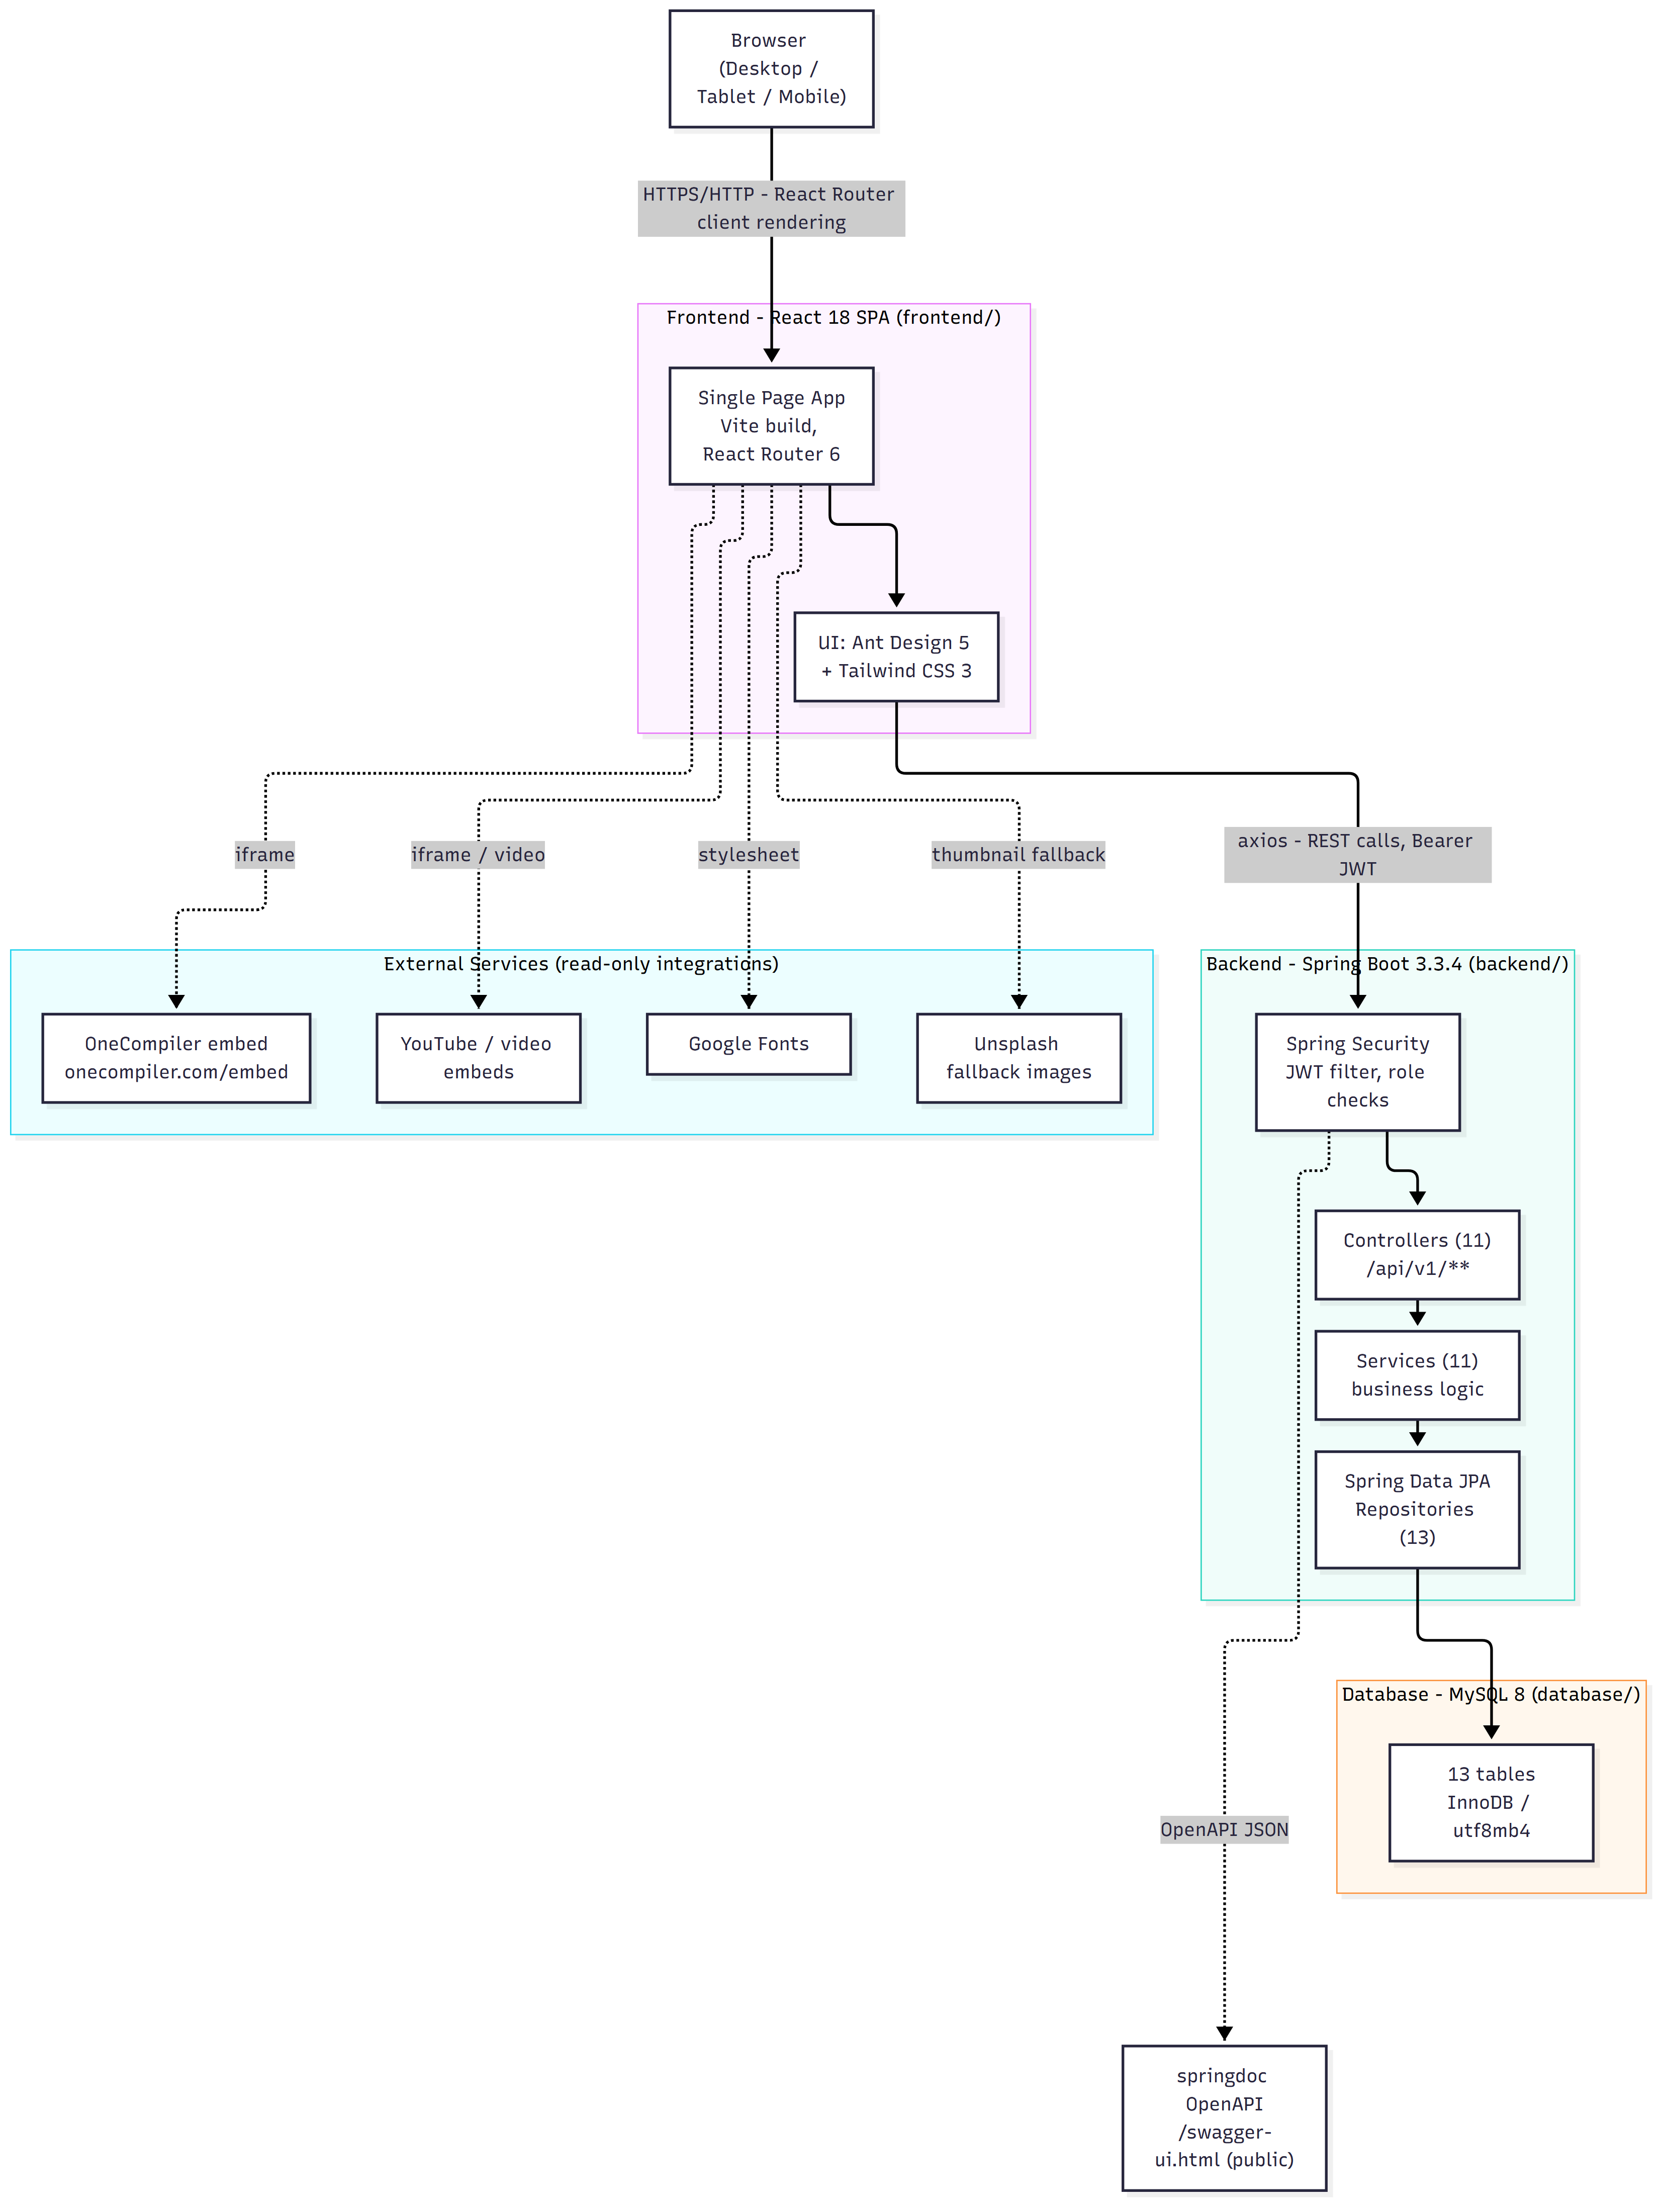
\includegraphics[width=0.72\textwidth]{diagrams/system-architecture.png}
    \caption{System architecture at a glance}
    \label{fig:system-architecture}
\end{figure}

\subsection{Current maturity}
\status{INFERRED}

\begin{itemize}
    \item \textbf{Working:} the end-to-end learning lifecycle passes an automated integration test; the frontend consumes the real API (no mock server); 61 automated tests exist across both tiers.
    \item \textbf{Not yet in place:} CI/CD, production deployment configuration, database migration tooling, licence file, rate limiting, monitoring/alerting, accessibility audit, SEO infrastructure (sitemap/structured data).
    \item \textbf{Repository signals:} 15 commits, active feature branches, contract-driven two-person workflow.
\end{itemize}

\subsection{Key limitations and risks (headline items)}
\status{IMPLEMENTED (verified findings)}

\begin{table}[H]
\centering
\caption{Headline limitations for leadership attention (full detail in Section~\ref{sec:security} and Section~\ref{sec:known-issues})}
\label{tab:exec-risks}
\begin{tabular}{@{}C{2.0cm}L{11.6cm}@{}}
\toprule
\textbf{Severity} & \textbf{Finding (evidence)} \\
\midrule
Critical & Open registration honours a caller-supplied \code{role} field -- an anonymous request can create an ADMIN account (\pathref{backend/src/main/java/com/example/lms/service/AuthService.java}) \\
Critical & Default admin credentials seeded on every fresh database (\code{admin@example.com}/\code{admin123}; \pathref{backend/src/main/java/com/example/lms/config/DataInitializer.java}) \\
High & Default JWT signing secret is committed to source; tokens are forgeable if the environment variable is unset \\
High & CORS allows any origin together with credentials (\pathref{SecurityConfig.java}) \\
Medium & Logout is client-side only -- the token stays valid for 24 hours \\
Medium & No pagination on any list endpoint; dashboard performs sequential per-enrolment requests \\
Medium & Several UI defects: footer links to non-existent routes, dashboard deep links do not switch tabs \\
Low & No CI/CD, no lint configuration, unused dependency (\code{canvas-confetti}) \\
\bottomrule
\end{tabular}
\end{table}

\subsection{Bottom line}
\status{INFERRED}

The repository delivers a credible, tested MVP of the full learn--assess--certify cycle with clear engineering governance (\pathref{CONTRACT.md}). Before any production exposure, the critical and high security findings above must be remediated and a deployment/CI pipeline must be established. These are recommendations, not current capabilities.
